%\newpage
\section{Storage Manager Hardware} 
\subsection{Overview} 
An overview of the Storage Manager (SM) hardware configuration is given in Figure~\ref{fig:system}. 
The HLT nodes are grouped in subfarms and connected to eight gigabit ethernet switches (Force10). Data from the HLT is sent to 8 SM nodes (Logger). 
%The input bandwidth is provided by 6 GigE links per Logger node providing. 
%Currently only 2 switches are connected with 2 GigE links to each Logger node.
% resulting in a total bandwitdh of 2GB/s. 
The Logger nodes are also connected to a GigE switch (Tier0) to provide connectivity to the Tier0 system at CERN.
The connection to the NexSan SATABeasts is provided through two Fibre Channel QLogic SanBox 5200 switches. Each NexSan SATABeast unit has two controllers with two fiber connections. If one controller fails, traffic can be switched to the second controller. The total network connectivity from the Logger nodes to the storage units is 8 time 2~Gb, such that the system is limited by the performance of the SATABeast controller. According to specification each NexSan SATABeast should be able to maintain 400MB/s write and 800MB/s read speed, if equipped with a sufficient number of disks.

% system overview
\begin{figure}[tbh]
\begin{center}  
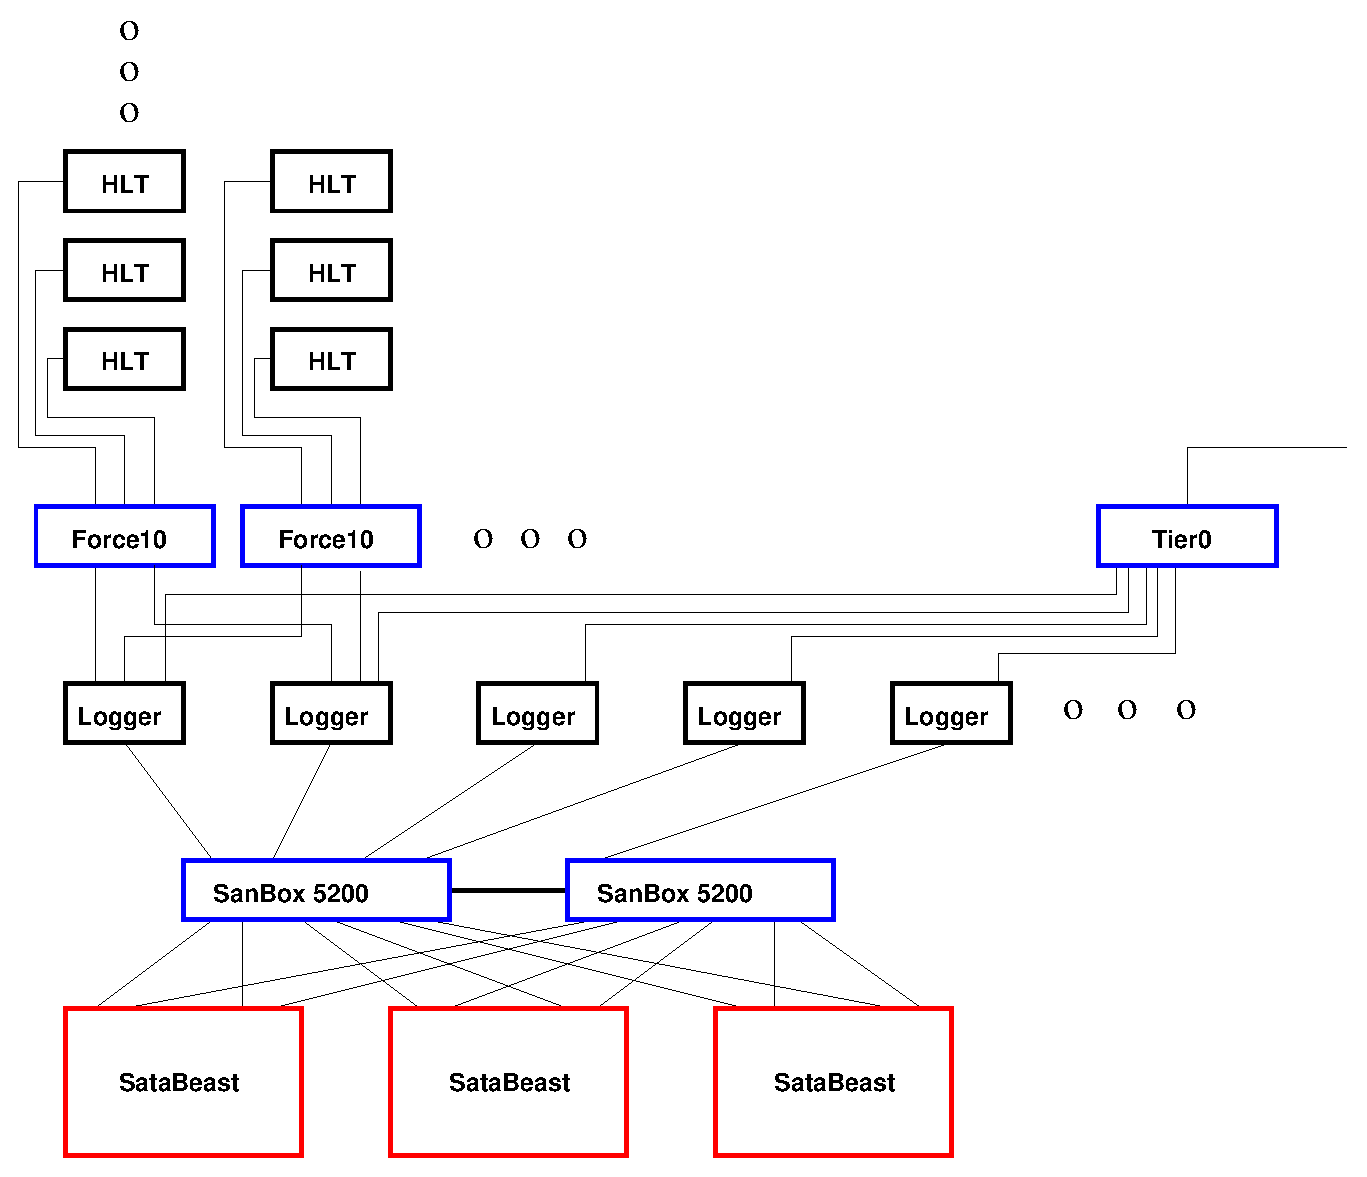
\includegraphics[width=1.0\textwidth]{Hardware/SMsystem.eps}
\caption{\emph{ Storage Manager system overview. }}
\label{fig:system}
\end{center}
\end{figure}  

%\newpage
% hardware components
\subsection{Hardware Components}
\subsubsection{Logger Nodes}
Logger nodes are standard Dell PC's PowerEdge 2950 with two dual-core Xeon processors and 4 GB RAM. Each node is equipped with a 4-port GbE card (Silicom PEG4i) and a fiber channel host bus adapter (QLogic QLE2460-CK). An additional PCI-e slot is available for an extra 4-port GbE card if needed. The same PC's are used for the CMS HLT farm.

\subsubsection{Fiber channel switch}
The fiber channel switches are used to connect the Logger nodes and the storage. Two QLogic SanBox 5200 switches are available. Each chassis includes sixteen 2Gb ports, plus a four-pack of high-speed 10Gb ISL ports of which one is used to connect the two switches.

\subsubsection{Storage Array}
The storage arrays are the SATABeast from NEXSAN. Currently, 3 SATABeasts are available with ten 750~GB Sata disks per array resulting in 21~TB storage. Each system has two controller with two 2~Gb ports.
The total number of disk slots available is 42 and the system can support Sata disks of up to 1~TB size. NexSan SATABeasts have been successfully deployed for the CDF Consumer Server Logger system in 2006.

% expected performance
\subsection{Expected Performance}
The proto-type system, currently installed in Cessy, has a storage capacity of 21~TB and is expected to be limited to 400MB/s per SataBeast for concurrent reads and writes. 

The HLT subfarm and the logger nodes are connected with 8 times 2~GbE links which can be extended to 8 times 6~GbE links using a second Silicom card. An additional switch could be used to connect all Logger nodes with all HLT subfarm to allow for easier system configurations.

The Tier0 switch and each Logger nodes will be connected with 2~GbE links.  

The proto-type system will already be able to provide a throughput of 1~GB/s. In 2008, shortly before we can expect the first collisions we plan to increase the storage capacity more than 100~TB by filling all available 126 slots with SATA disk.

To increase the storage capacity to the design capacity of 250~TB, additional SataBeast have to be added. With 3 additional storage arrays the system can be increased to more than 200~TB. This addition will also increase the IO bandwidth. 

% Commissioning Plans
\subsection{Commissioning Plans}
The proto-type system has been installed during the summer 2007 and is currently being configured. Connectivity and small scale system tests will be carried out in November 2007. End of November the system will be used for a Global Run commissioning exercise. End of December performance tests will be carried out to benchmark the system performance. 

% cost and upgrade plans
\subsection{Cost and Upgrade Plans}
Table~\ref{tab:proto} shows the costs for the proto-type system with the exception of the Logger nodes, Silicom cards and fibers, which where ordered together with the nodes used for the HLT farm or a database project. In total \$80k were spend on the proto-type system. Costs and cost projections for Storage Manager hardware are summarized in Table~\ref{tab:costs}. With an additional \$51k, the storage capacity can be increased to more than $100$~TB. To increase the storage capacity and the connectivity even more, additional SataBeasts are needed. In order to increase the capacity to more than $200$~TB an investment of \$117k is needed. Given a limited lifetime for disks and host bus adapter, we assume that about 20\% have to be replaced after 3 years. 
The cost projections are given assuming spring 2007 prices for the SATABeast and 750~GB SATA disks. 

\begin{table}[!ht]
\begin{center}
\begin{tabular}{l|r|r}
year & cost    & product \\\hline\hline
2007 & \$66k   & 3 SataBeasts with 10 disks  \\\hline
2007 & \$6k    & 2 QLogic switches  \\\hline
2007 & \$8k    & 8 QLogic HBAs \\\hline
2007 &         & 8 Dell PowerEdge 2950 \\\hline
2007 &         & 8 Silicom PEG4i \\\hline
2007 &         & 20 2m fiber \\\hline\hline
\end{tabular}
\caption{Proto-type system costs.}
\label{tab:proto}
\end{center}
\end{table}

\begin{table}[!ht]
\begin{center}
\begin{tabular}{l|r|r}
year & cost    & product \\\hline\hline
2007 & \$80k   & proto-type system \\\hline
2008 & \$51k   & 96 SATA disks  \\\hline
2009 & \$66k   & 3 SataBeasts with 10 disks  \\\hline
2009 & \$51k   & 96 SATA disks  \\\hline
2010 & \$17k   & Hardware replacement  \\

\end{tabular}
\caption{Storage Manager system costs.}
\label{tab:costs}
\end{center}
\end{table}
